
\fancyhf{}
\fancyhead[c]{Chapter 6. Supplementary Materials}% <- added
\fancyfoot[R]{\thepage\ifodd\value{page}\else\hfill\fi}
%\fancyhead[L]{\ifodd\value{page}\relax\else\hfill\fi Ch \thechapter}
%\renewcommand\headrulewidth{0pt}% default ist .4pt
\renewcommand{\plainheadrulewidth}{.4pt}% default is 0pt


\section{Supplementary materials for Chapter 2}

\clearpage
\newpage

\section{Waveform and Action Potential properties manifold \\ comparison }
\begin{figure}[!htpb]
    \centering
    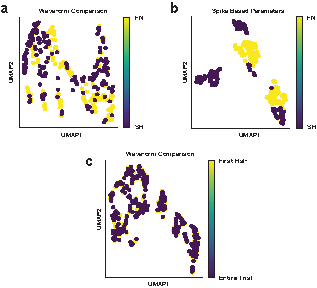
\includegraphics[width=0.8\linewidth]{Figures/Ch_2/appendix1.pdf}
    \caption{(\textbf{a}) Overlaid UMAP representation FN and SH waveforms from 186 neuron used in classification. The waveform shapes are different between SH and FN protocols.(\textbf{b}) FN and SH Action potential parameters used for classification projected together on the same space. The Action potential properties are different between FN and SH protocols. The SH Action potential properties show a bigger spread than FN properties. (\textbf{c}) UMAP projection of averaged Waveform comparison between the first half and the entire trial. The average waveform shape doesn't change as a result of trial length.  }
    \label{first:app1}
\end{figure}
\clearpage

\newpage


\section{Louvain vs Ensemble Clustering for Graphs (ECG) algorithm comparison }
\begin{figure}[!htpb]
    \centering
    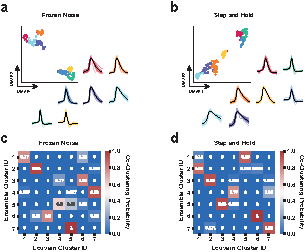
\includegraphics[width=\linewidth]{Figures/Ch_2/appendix2.pdf}
    \caption{(\textbf{a}) UMAP embedding of FN waveforms colored with cluster labels found using Ensemble clustering, with original waveforms in the same color as the respective color. 7 clusters were observed, the same number as in the case of the Louvain community method. (\textbf{b}) UMAP embedding of SH waveforms colored with cluster labels found using Ensemble clustering, with original waveforms in the same color as the respective color. 7 clusters were observed, the same number as in the case of the Louvain community method. (\textbf{c}) Heatmap showing the correspondence between Louvain and Ensemble clustering for graph on FN waveforms. Clusters using the Louvain community detection algorithm show a high correspondence with the clusters obtained using Ensemble clustering for the graph method. (\textbf{d}) Heatmap showing the correspondence between Louvain and Ensemble clustering for graph on SH waveforms. Clusters using the Louvain community detection algorithm show a high correspondence with the clusters obtained using Ensemble clustering for the graph method.}
    \label{first:app2}
\end{figure}
% \begin{figure}
%  \end{figure}
% \clearpage
\newpage

% \label{first:app3}
\section{Cluster stability after leaving one attribute out at a time}
\begin{figure}[!htpb]
    \centering
    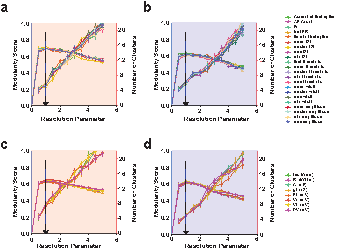
\includegraphics[width=\linewidth]{Figures/Ch_2/appendix3.pdf}
    \caption{(\textbf{a-b}) Stability of clusters for action potential attributes leaving one attribute out for excitatory and Inhibitory sets. The clustering was performed 25 times with random 80\% samples for resolution attributes ranging from 0.0 to 1, the mean and standard deviation of the resulting number of clusters and modularity score are plotted. For the chosen resolution parameter (1.0), the cluster numbers fluctuate between 5-7. The cluster number fluctuates more for the excitatory set (left) than the Inhibitory set (right) (\textbf{c-d}) Stability of clusters for biophysical attributes leaving one attribute out for excitatory and Inhibitory sets. The clustering was performed 25 times with random 90\% samples for resolution parameters ranging from 0.0 to 1, the mean and standard deviation of the resulting number of clusters and modularity score are plotted. For the chosen resolution parameter (1.0), the excitatory population fluctuates between 6-8. On the contrary, the Inhibitory population doesn't show any fluctuation.}
    \label{first:app3}
\end{figure}
\clearpage

\newpage

% \label{first:app4}

\section{Diversity of firing rate and AP half-width}
\begin{figure}[!htpb]
    \centering
    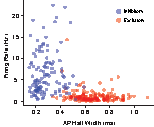
\includegraphics[width=\linewidth]{Figures/Ch_2/appendix4.pdf}
    \caption{Firing rate vs AP half-width between excitatory (red) and inhibitory (blue) populations. The excitatory population has a lower firing rate and higher AP width. The Inhibitory population has a lower AP width and higher firing rate.}
    \label{first:app4}
\end{figure}


\newpage
% \label{first:app5}
\section{STA Heterogeneity}
\begin{figure}[!htpb]
    \centering
    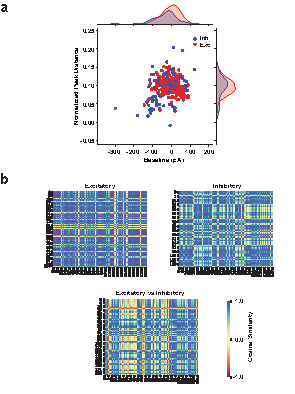
\includegraphics[width=0.8\linewidth]{Figures/Ch_2/appendix5.pdf}
    \caption{{(\textbf{a}) The scatter plot shows the baseline added to the theoretical input vs the Peak distance of the STA. The excitatory population has a higher baseline and higher peak distance. The variance for both baseline and peak distance seems higher for the excitatory population than inhibitory population. (\textbf{b}) The STA cosine similarity is for the excitatory population (top left), the STA cosine similarity is for the inhibitory population (top right), and the STA cosine similarity is between the excitatory and inhibitory populations. The excitatory population has higher similarity than the inhibitory population.}}
    \label{first:app5}
\end{figure}


\clearpage
\newpage
% \label{first:app6}

\section{Cluster assignment likelihood across attributes}
\begin{figure}[!htpb]
    \centering
    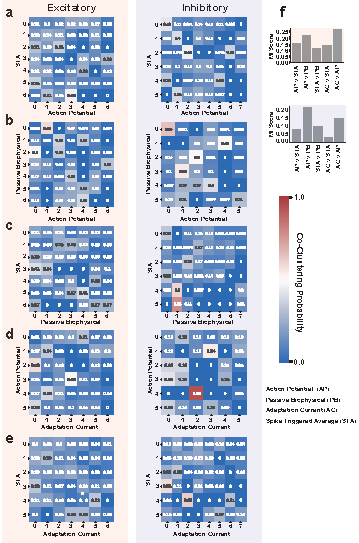
\includegraphics[width=0.8\linewidth]{Figures/Ch_2/appendix6.pdf}
    \caption{(\textbf{a-e}) Heatmap showing the likelihood for neuron clustering in attribute 1 clustering }
    \label{first:app6}
\end{figure}
\begin{figure}
 in one of the clusters in attribute 2 for excitatory (left) and inhibitory (right) population. For each attribute (Action potential, Passive biophysical, STA, Adaptation current ($\eta$), none of the clusters show a high likelihood to be clustering in another attribute. (f) Cluster label comparison between modularity pairs using Mutual information score for excitatory and inhibitory population. None of the pairs reach the modularity of 0.25 showing that neurons cluster differently across attribute sets.
\end{figure}
\clearpage
\newpage

\section{Supplementary materials for Chapter 3}

\newpage


\begin{figure}
    \centering
    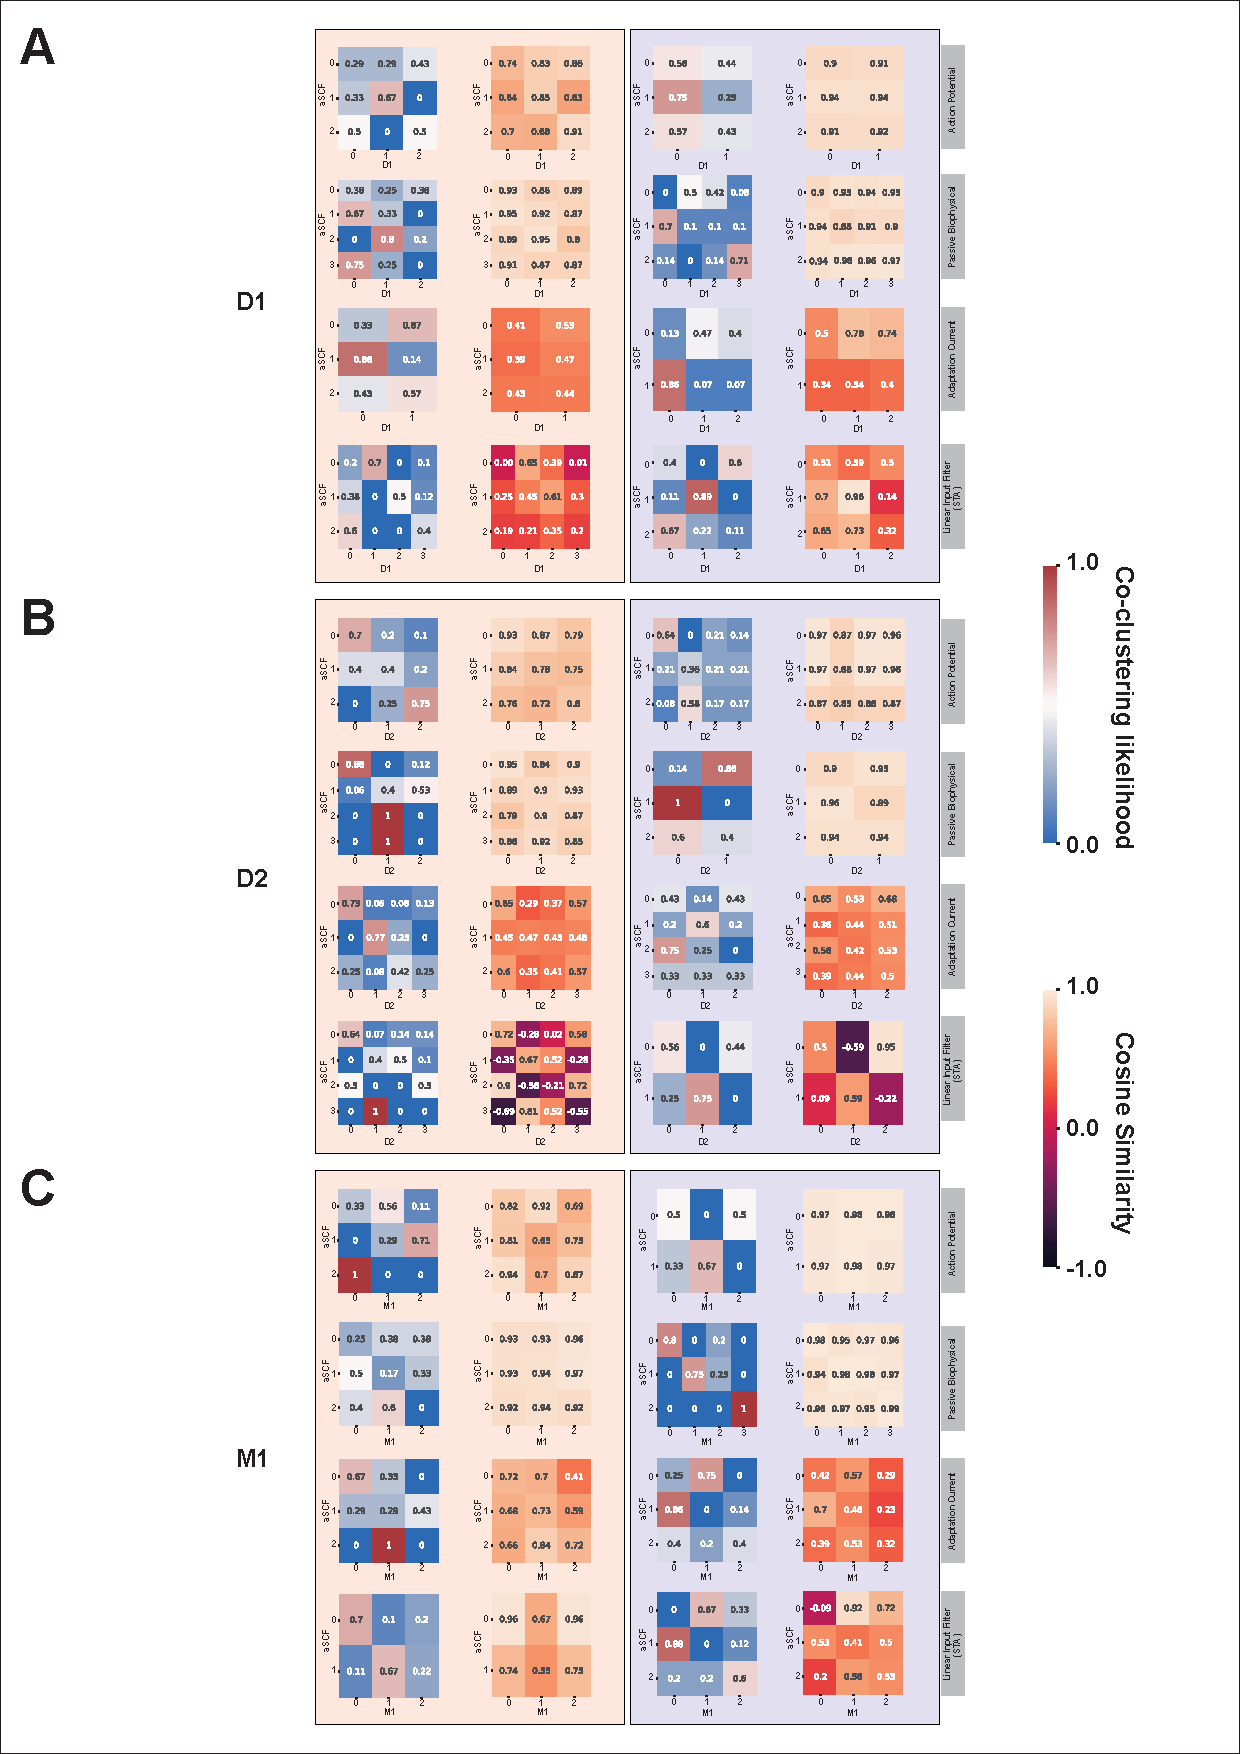
\includegraphics[width=\linewidth]{Figures/Ch_3/Appendix1.pdf}
    \caption{\textbf{Clustering likelihood matrix and cosine similarity across labels shifts for all four properties as a result of neuromodulation for D1-R, D2-R and M1-R}}
    \label{fig:S1_ref}
\end{figure}
\newpage

\begin{figure}
   Top panel shows the cluster likelihood and cosine similarity for D1 vs aCSF trials. Middle shows the cluster likelihood and cosine similarity for D2 vs aCSF trials. Bottom shows the cluster likelihood and cosine similarity for M1 vs aCSF trials.
\end{figure}
\clearpage

\newpage
\begin{figure}
    \centering
    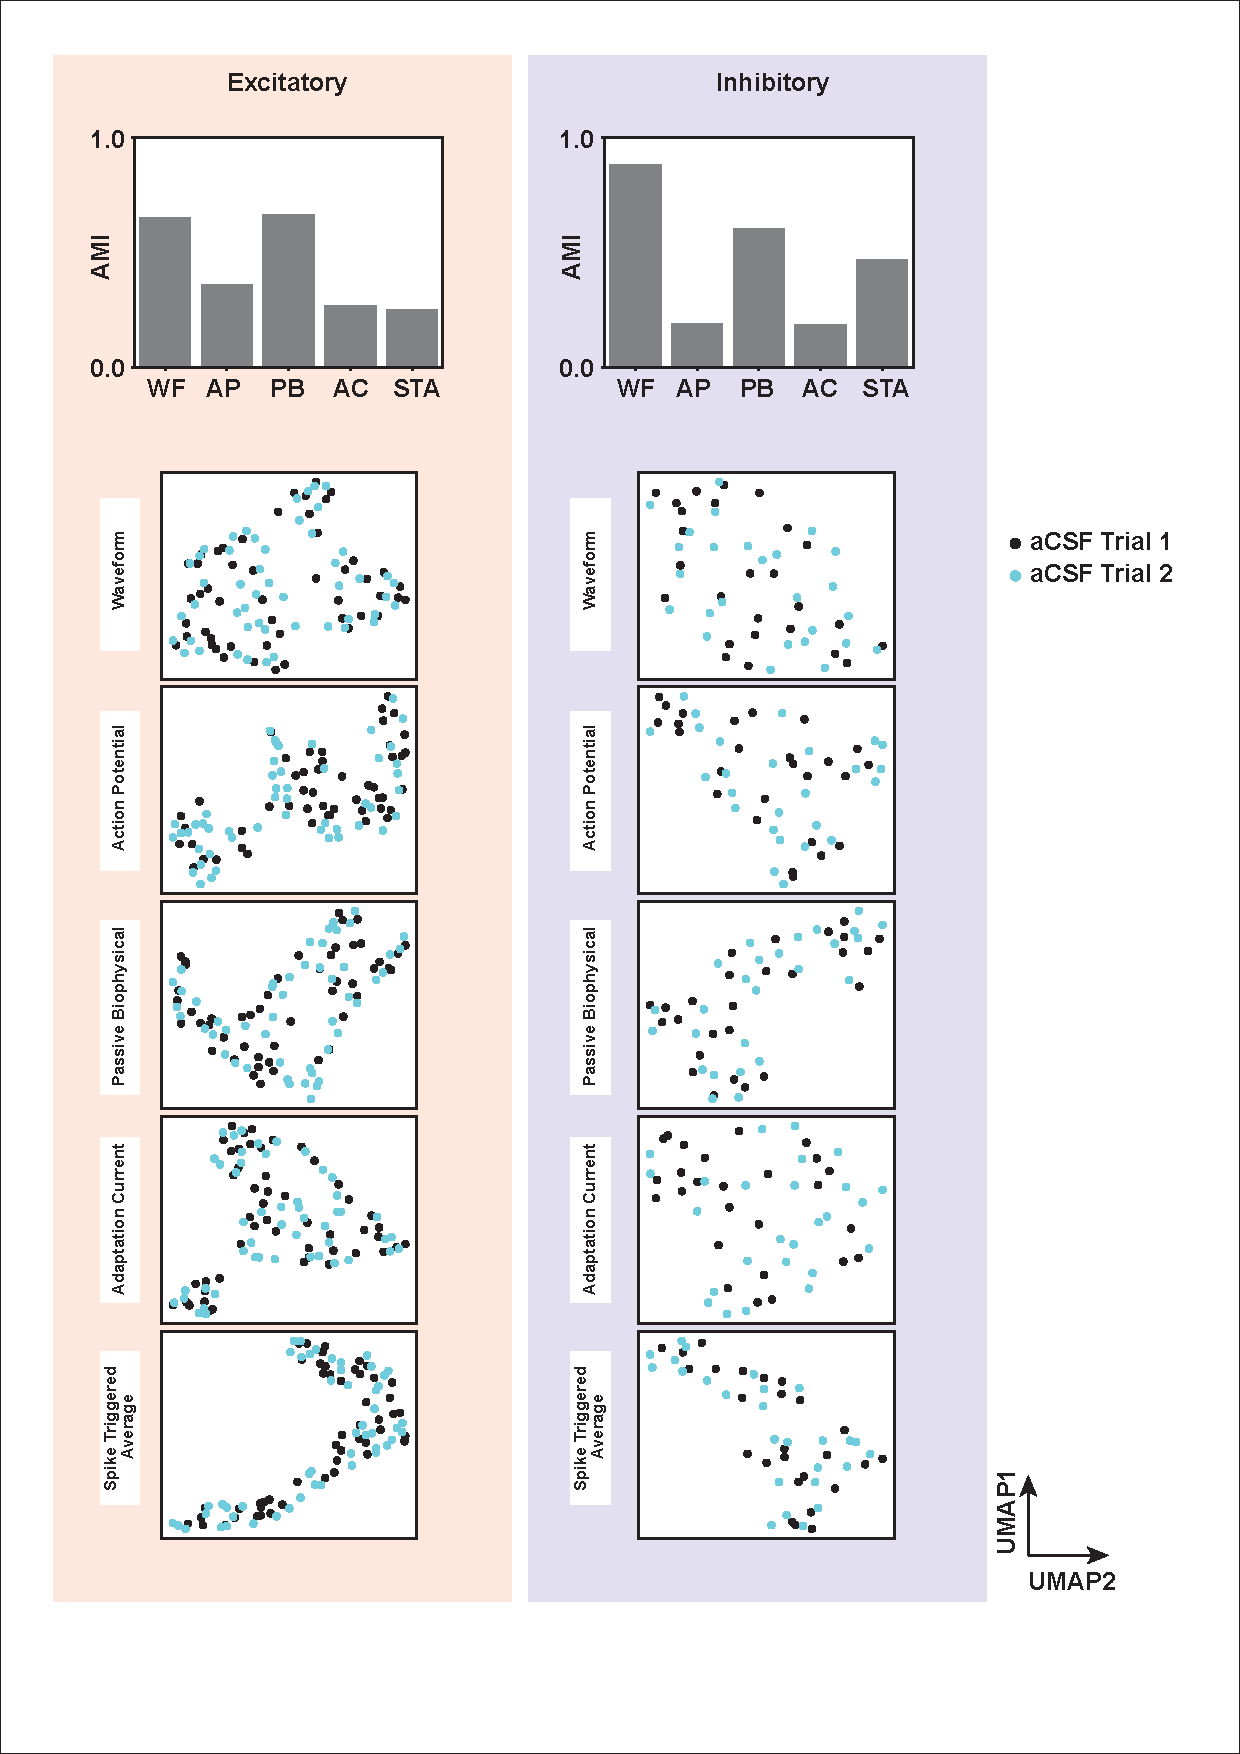
\includegraphics[width=\linewidth]{Figures/Ch_3/Appendix2.pdf}        
    \caption{\textbf{Comparison of aCSF trial 1 vs trial 2 clustering and manifold}}
    \label{fig:S2}
\end{figure}

\begin{figure}
Left and right histograms on top the AMI score between cluster IDs found for aCSF trial 1 vs aCSF trial 2. Waveforms and passive biophysical properties were found to be consistent across the two trials as these properties are not strongly dependent input dynamics. The UMAP plots show the alignment for aCSF trial 1 vs aCSF trial 2.
\end{figure}
\clearpage


\newpage
\begin{figure}
    \centering
    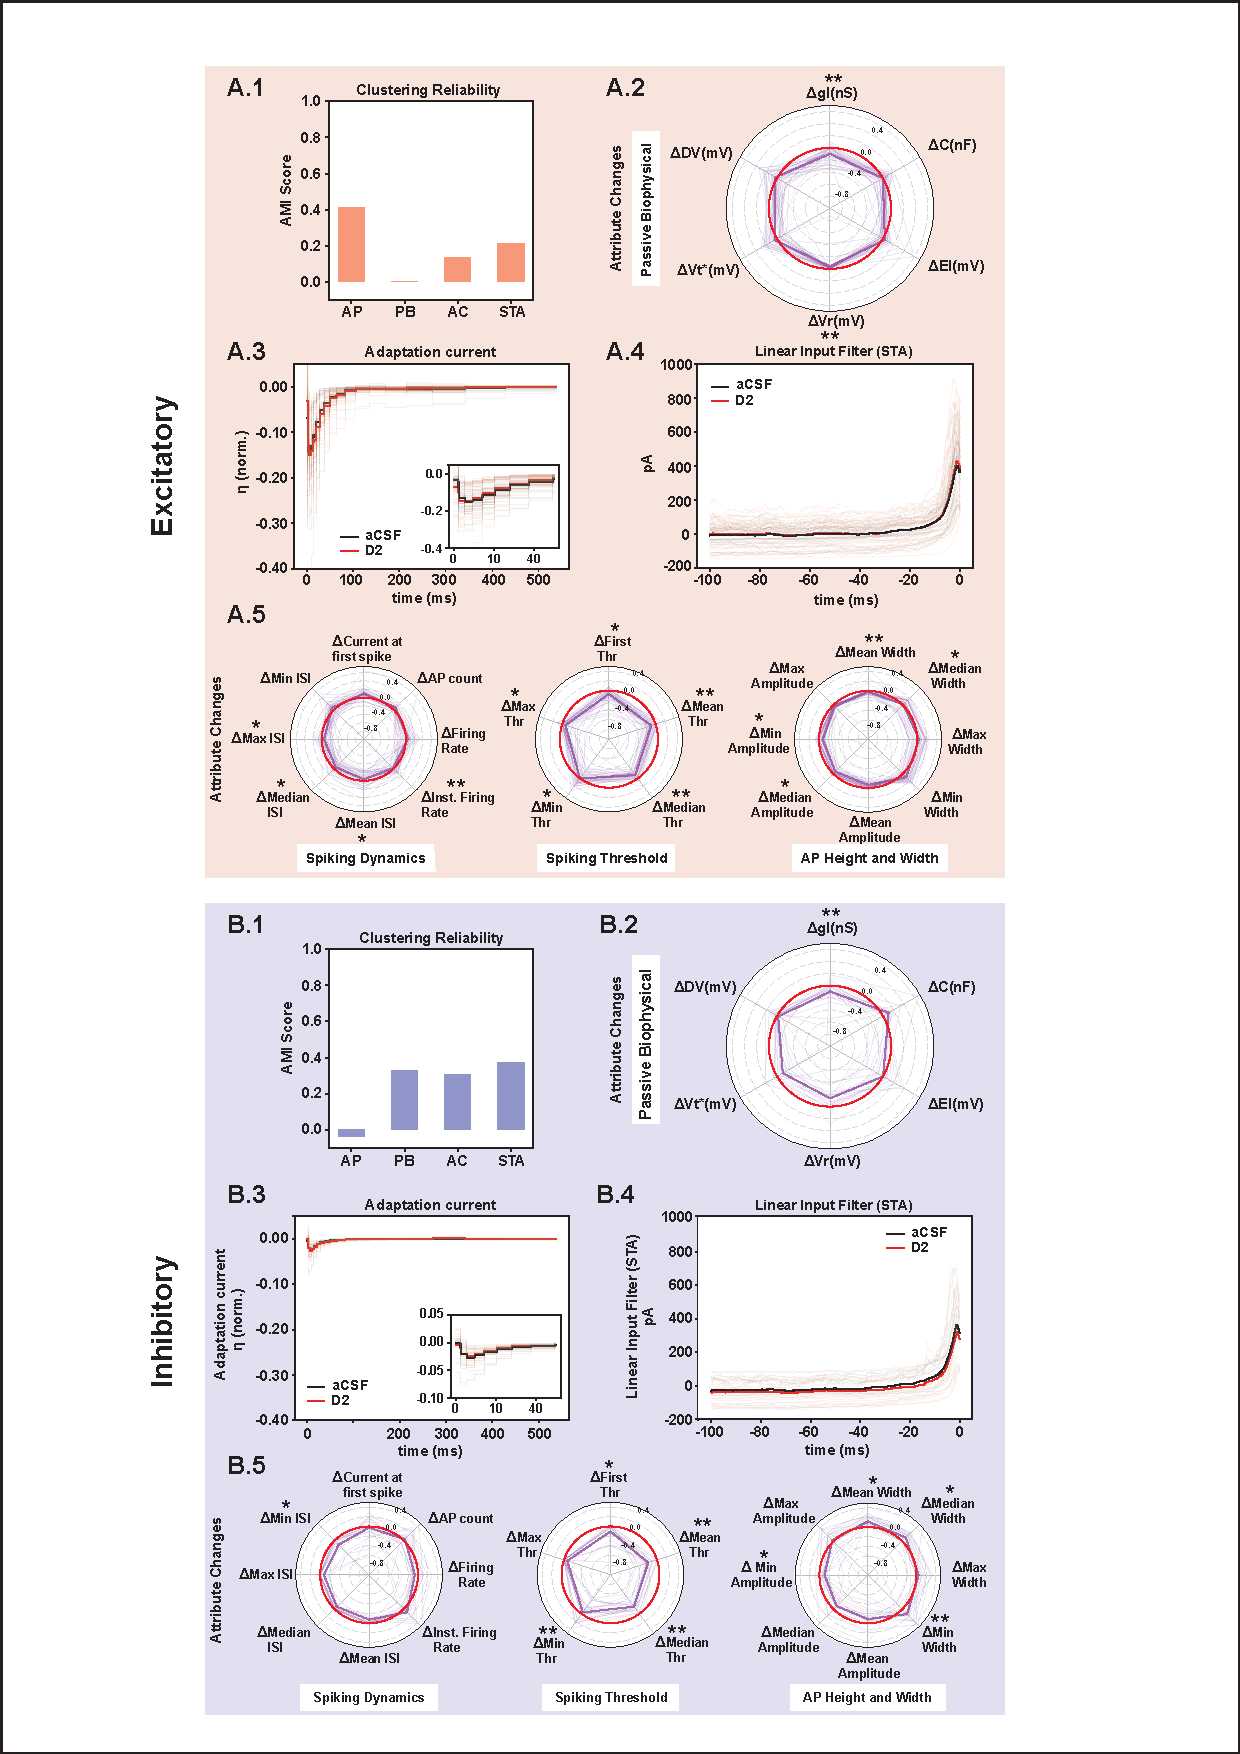
\includegraphics[width=\linewidth]{Figures/Ch_3/Appendix3.pdf}
    \caption{\textbf{D2 receptor activation changes functional clustering and attributes for both excitatory and inhibitory neurons.} }
    \label{fig:S3_ref}
\end{figure}
\newpage
    
\begin{figure}
(\textbf{A.1}) Histogram shows the adjusted mutual information score between the clustering labels obtained for aCSF and D2 trials, the histogram shows a shift in cluster identities as a result of D2 receptor activation across four attributes. (\textbf{A.2}) shows the change in passive parameters with respect to control as a result of D2 receptor activation, normalized by the control trial values. With the mean marked represented with a thick line. (\textbf{A.3}) shows the adaptation current for control (black) and D2 (red), the mean is represented with darker curves. The adaptation current profiles between D2 and aCSF trials were found to be similar. The rise time as well the peak adaptation current between aCSF and D2 were found to be non-significant (see Appendix  \ref{fig:S5}). (\textbf{A.4}) shows the spike triggered average profile for aCSF (black) and D2 (red) trials, the mean is represented with a thick line. (\textbf{A.5}) shows the change in action potential attribute sets with respect to control as a result of D2 receptor activation, normalized by the control trial values. With the mean marked represented with a thick line and the zero line is colored in red. The significant features are marked. \textbf{B.1-5} Same analysis repeated for inhibitory neurons. * $p<0.05$, ** $p<0.001$, *** $p<0.0001$.

\end{figure}
\clearpage

\newpage
\begin{figure}
    \centering
    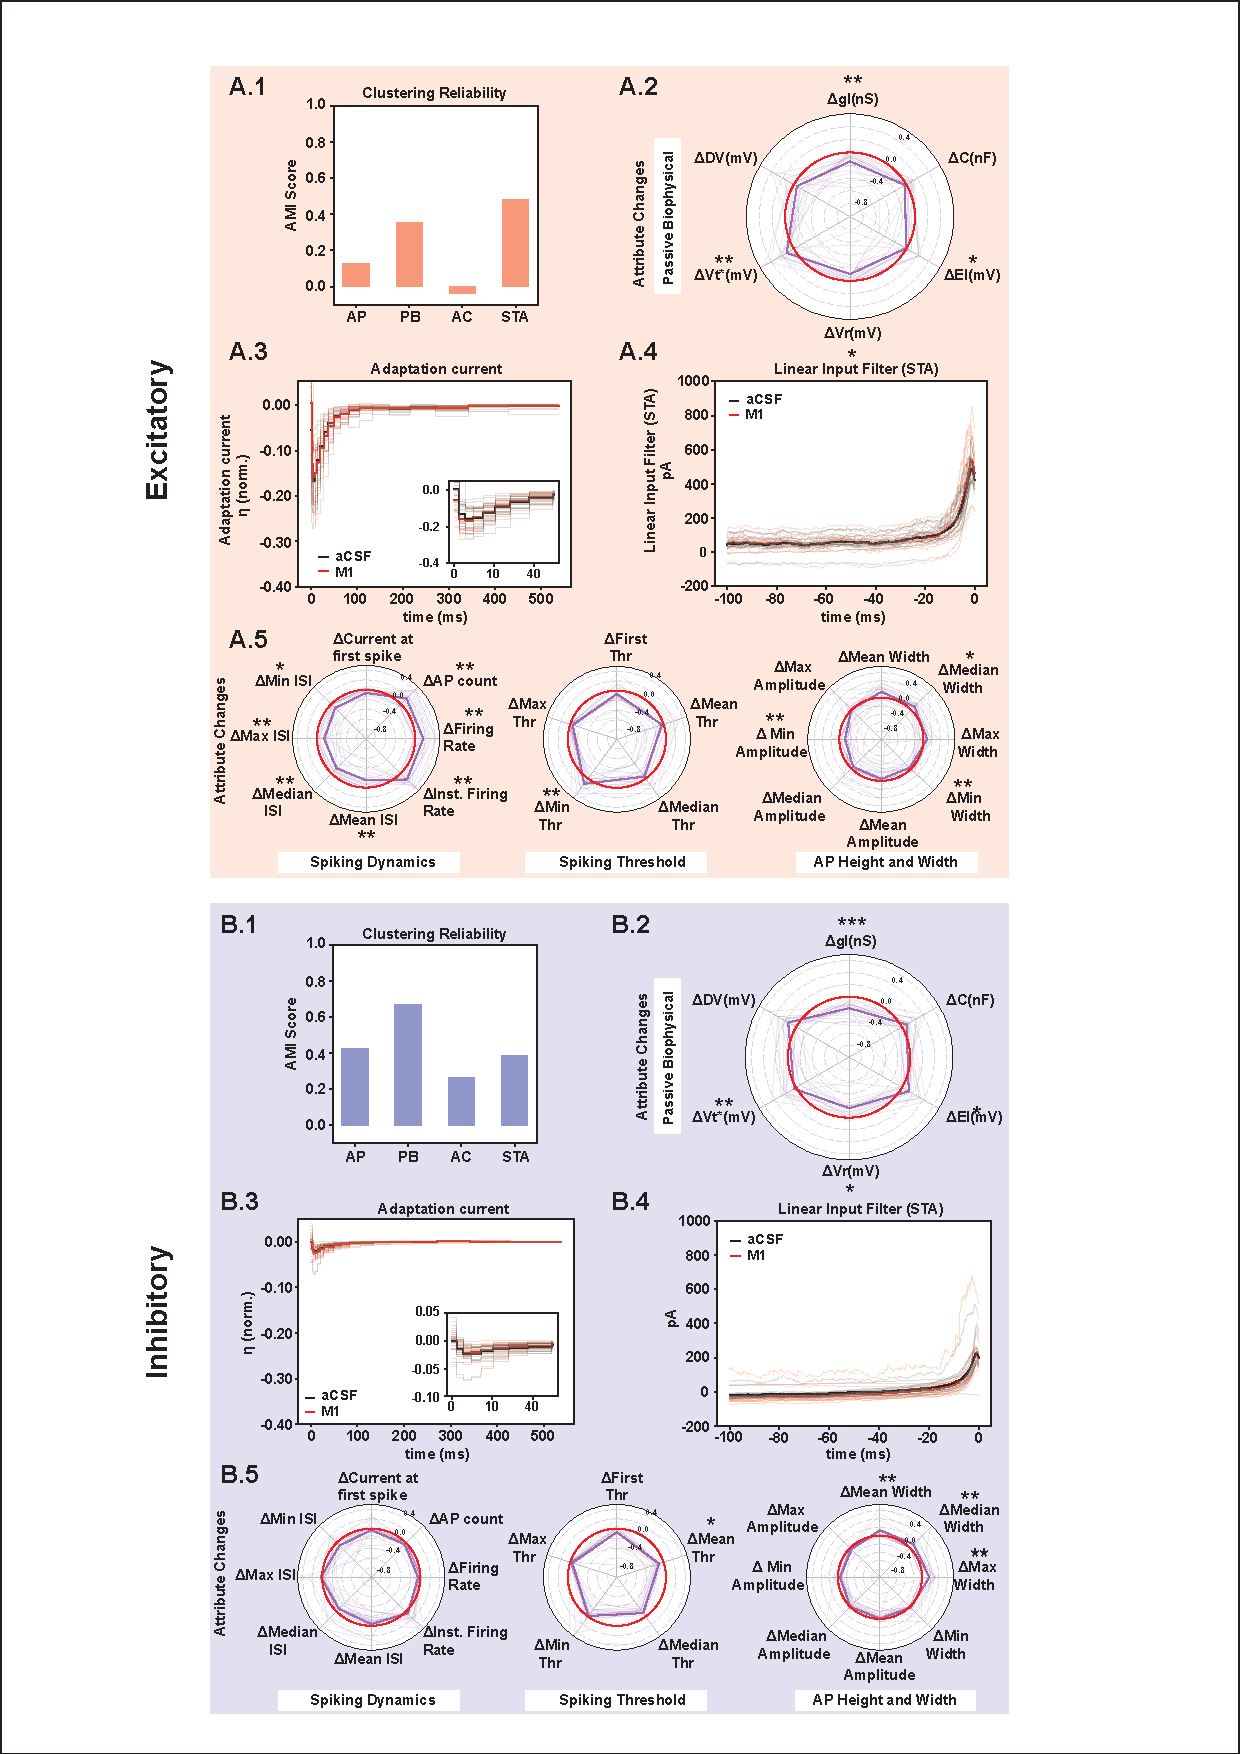
\includegraphics[width=\linewidth]{Figures/Ch_3/Appendix4.pdf}
    \caption{\textbf{M1 receptor activation changes functional clustering and attributes for both excitatory and inhibitory neurons.}}
    \label{fig:S4_ref}
\end{figure}
\newpage

\begin{figure}
(\textbf{A.1}) Histogram shows the adjusted mutual information score between the clustering labels obtained for aCSF and M1 trials, the histogram shows a shift in cluster identities as a result of M1 receptor activation across four attributes. (\textbf{A.2}) shows the change in passive parameters with respect to control as a result of M1 receptor activation, normalized by the control trial values. With the mean marked represented with a thick line. (\textbf{A.3}) shows the adaptation current for control (black) and M1 (red), the mean is represented with darker curves. The adaptation current profiles between M1 and aCSF trials were found to be similar. (\textbf{A.4}) shows the spike triggered average profile for aCSF (black) and M1 (red) trials, the mean is represented with a thick line. (\textbf{A.5}) shows the change in action potential attribute sets with respect to control as a result of M1 receptor activation, normalized by the control trial values. With the mean marked represented with a thick line and the zero line is colored in red. \textbf{B.1-5} Same analysis repeated for inhibitory neurons. * $p<0.05$, ** $p<0.001$, *** $p<0.0001$.

\end{figure}
\clearpage




\newpage
\begin{figure}
    \centering
    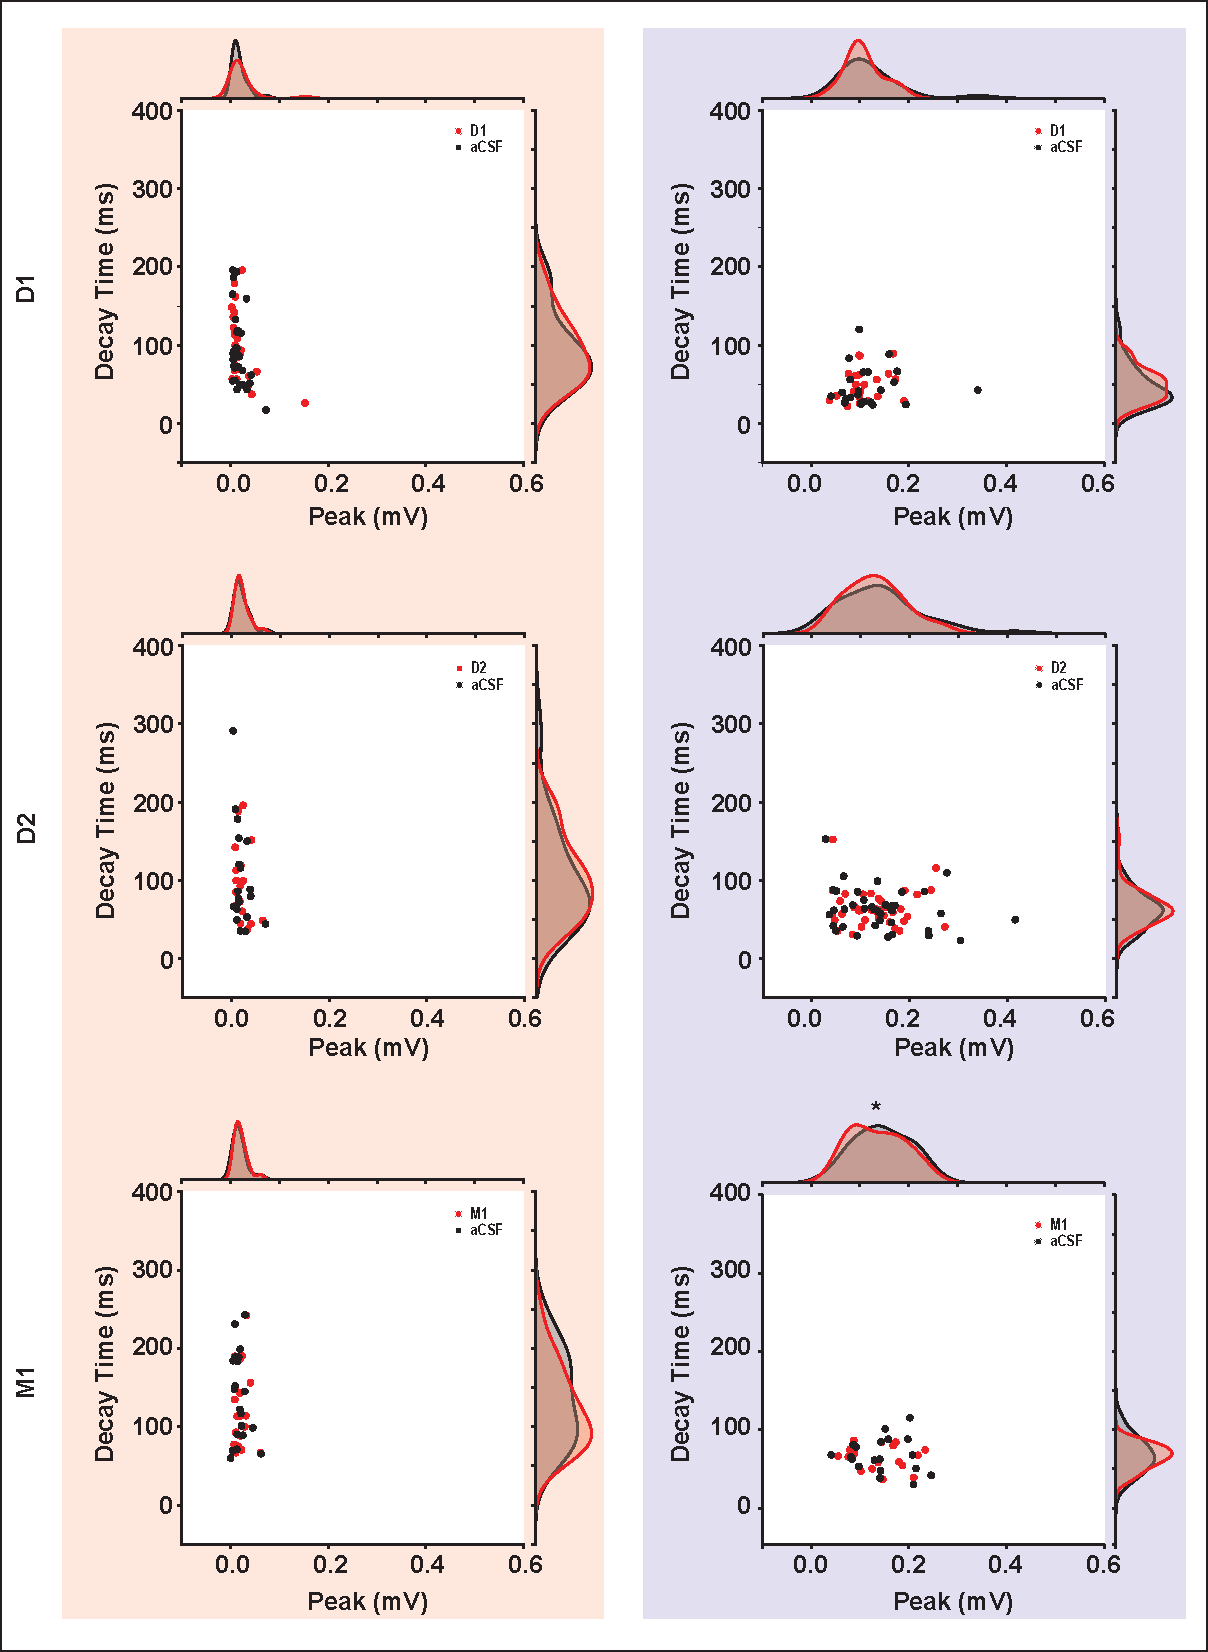
\includegraphics[width=0.9\linewidth]{Figures/Ch_3/Appendix5.pdf}
    \caption{\textbf{Adaptation current peaks and decay times are not strongly altered by D1, D2 and M1 modulation} The scatter plots show the normalized peaks of the AC curve on the x-axis and the decay time for D1, D2 and M1 vs aCSF trials. The red panel represents excitatory and blue panel represents inhibitory.  * $p<0.05$, ** $p<0.001$, *** $p<0.0001$.}
    \label{fig:S5}
\end{figure}

\newpage

\begin{figure}
    \centering
    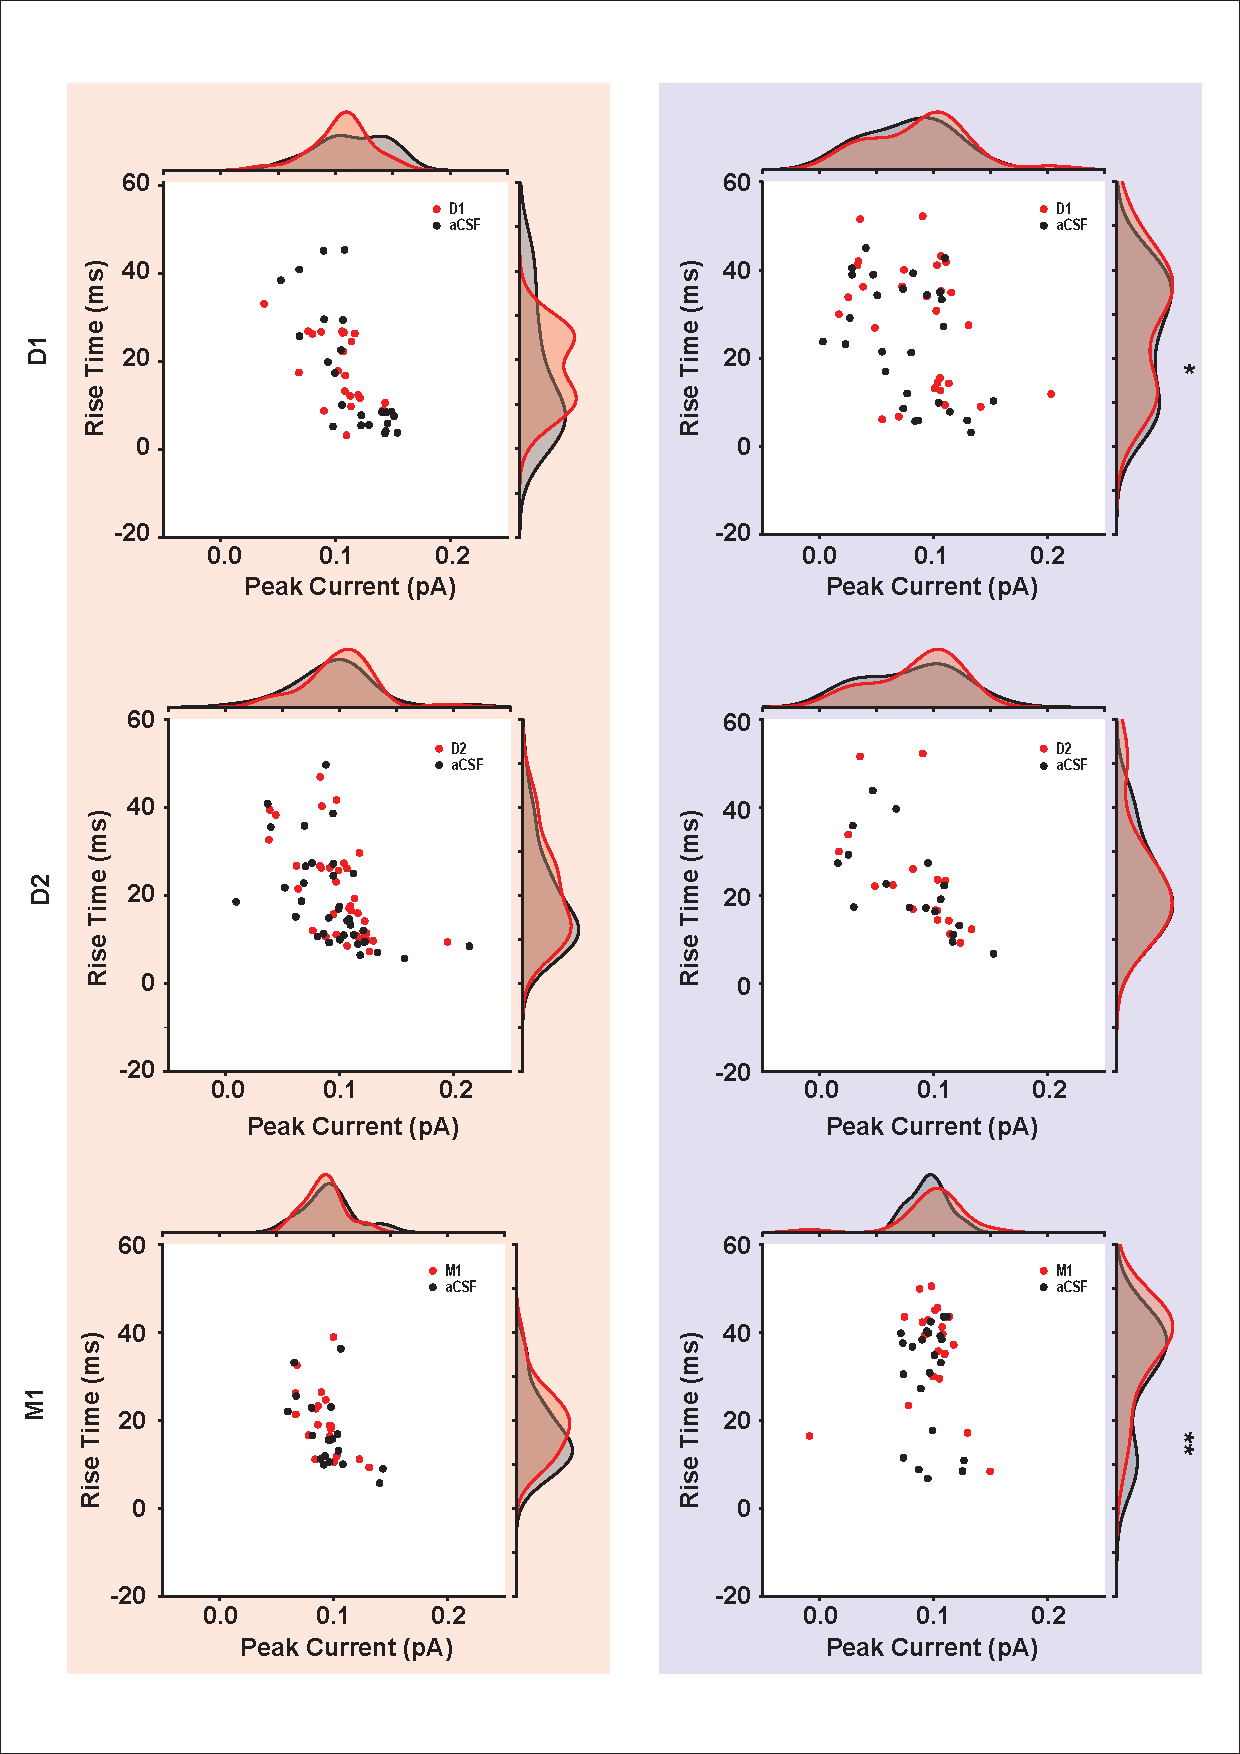
\includegraphics[width=0.9\linewidth]{Figures/Ch_3/Appendix6.pdf}
    \caption{\textbf{Spike triggered average peaks and decay times are modestly altered by D1, D2 and M1 modulation} The scatter plots show the normalized peaks of the STA curve on the x-axis and the decay time for D1, D2 and M1 vs aCSF trials. The red panel represents excitatory and blue panel represents inhibitory population.  * $p<0.05$, ** $p<0.001$, *** $p<0.0001$}
    \label{fig:S6}
\end{figure}
\newpage

\begin{figure}
    \centering
    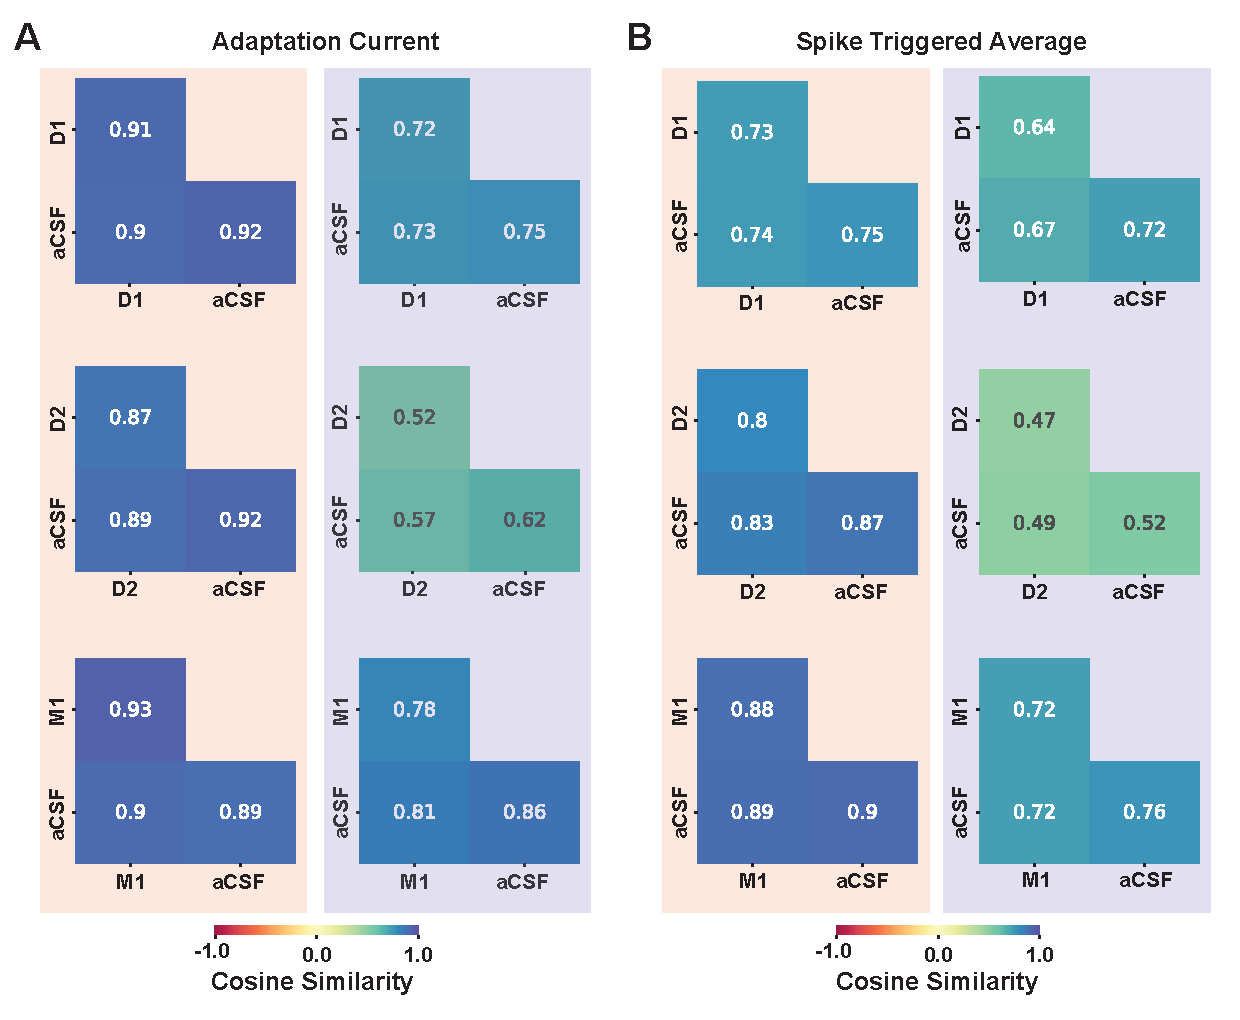
\includegraphics[width=\linewidth]{Figures/Ch_3/Appendix7.pdf}
    \caption{\textbf{Average cosine similarity across and within aCSF-Agonist trials vary in a cell-type specific manner.} (\textbf{A}) Heatmaps show the average AC similarity for excitatory (red background) and inhibitory (blue background) for D1, D2 and M1 vs aCSF trials. (\textbf{B}) Heatmaps show the average STA similarities for excitatory (red background) and inhibitory (blue background) for D1, D2 and M1 vs aCSF trials.}
    \label{fig:S7}
\end{figure}

\newpage

\begin{figure}
    \centering
    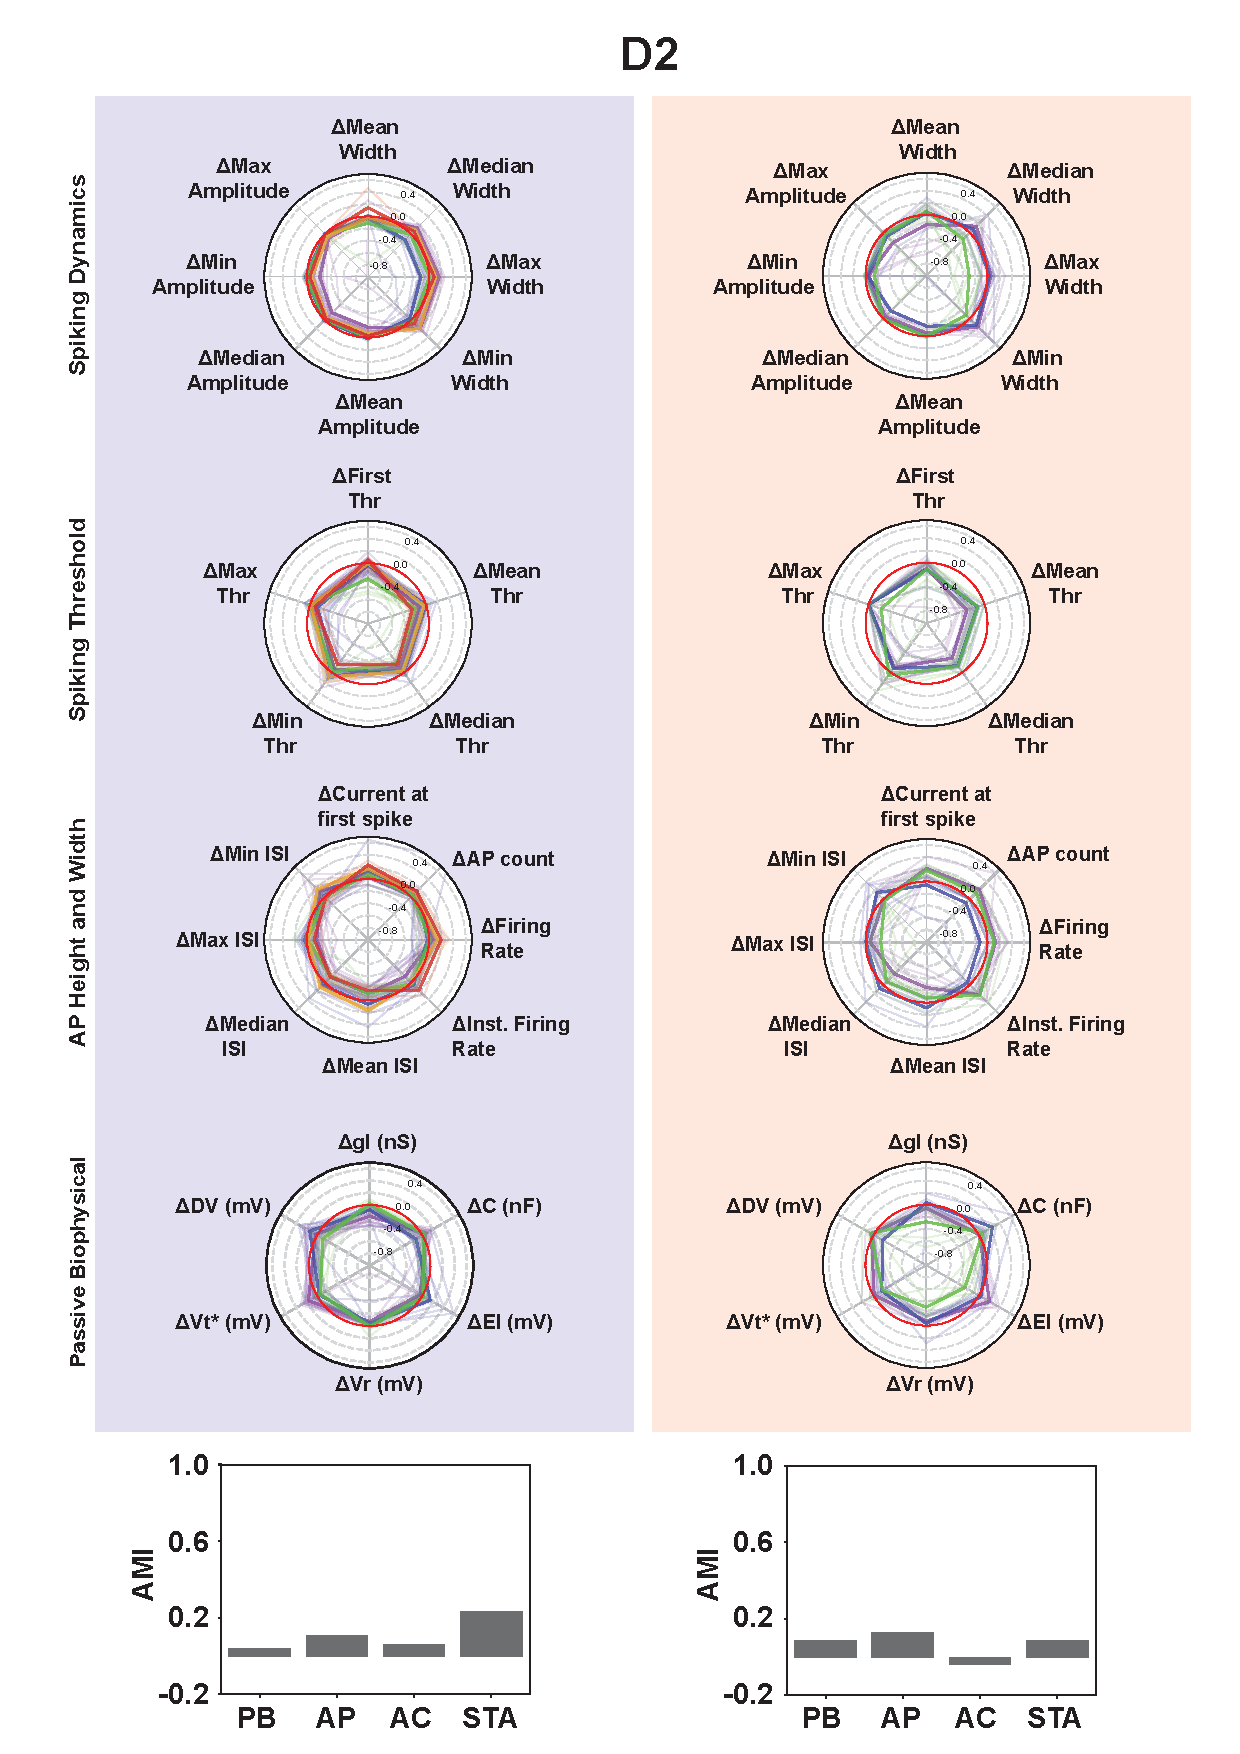
\includegraphics[width=0.9\linewidth]{Figures/Ch_3/Appendix8.pdf}
      \caption{\textbf{Clustering based on differences between control and D2 for action potential and passive biophysical attributes reveals subgroups of neurons getting modulated differently as a result of D2-R activation.}}
    \label{fig:S8}
\end{figure}

\begin{figure}
The polar plots show the clusters based on difference values between D2 and aCSF trials for action potential (subdivided into spiking dynamics, spiking threshold and AP height and width) and passive biophysical properties for both, excitatory (red background) and inhibitory (blue background). Each neuron is represented with a thin line and Coloured with their respective cluster label. The mean for each cluster is represented with a thick line. The histogram at the bottom shows the AMI score between cluster labels using aCSF trials and the cluster labels based on difference between D2 and aCSF trials.   
\end{figure}

\clearpage
\newpage

\begin{figure}
    \centering
    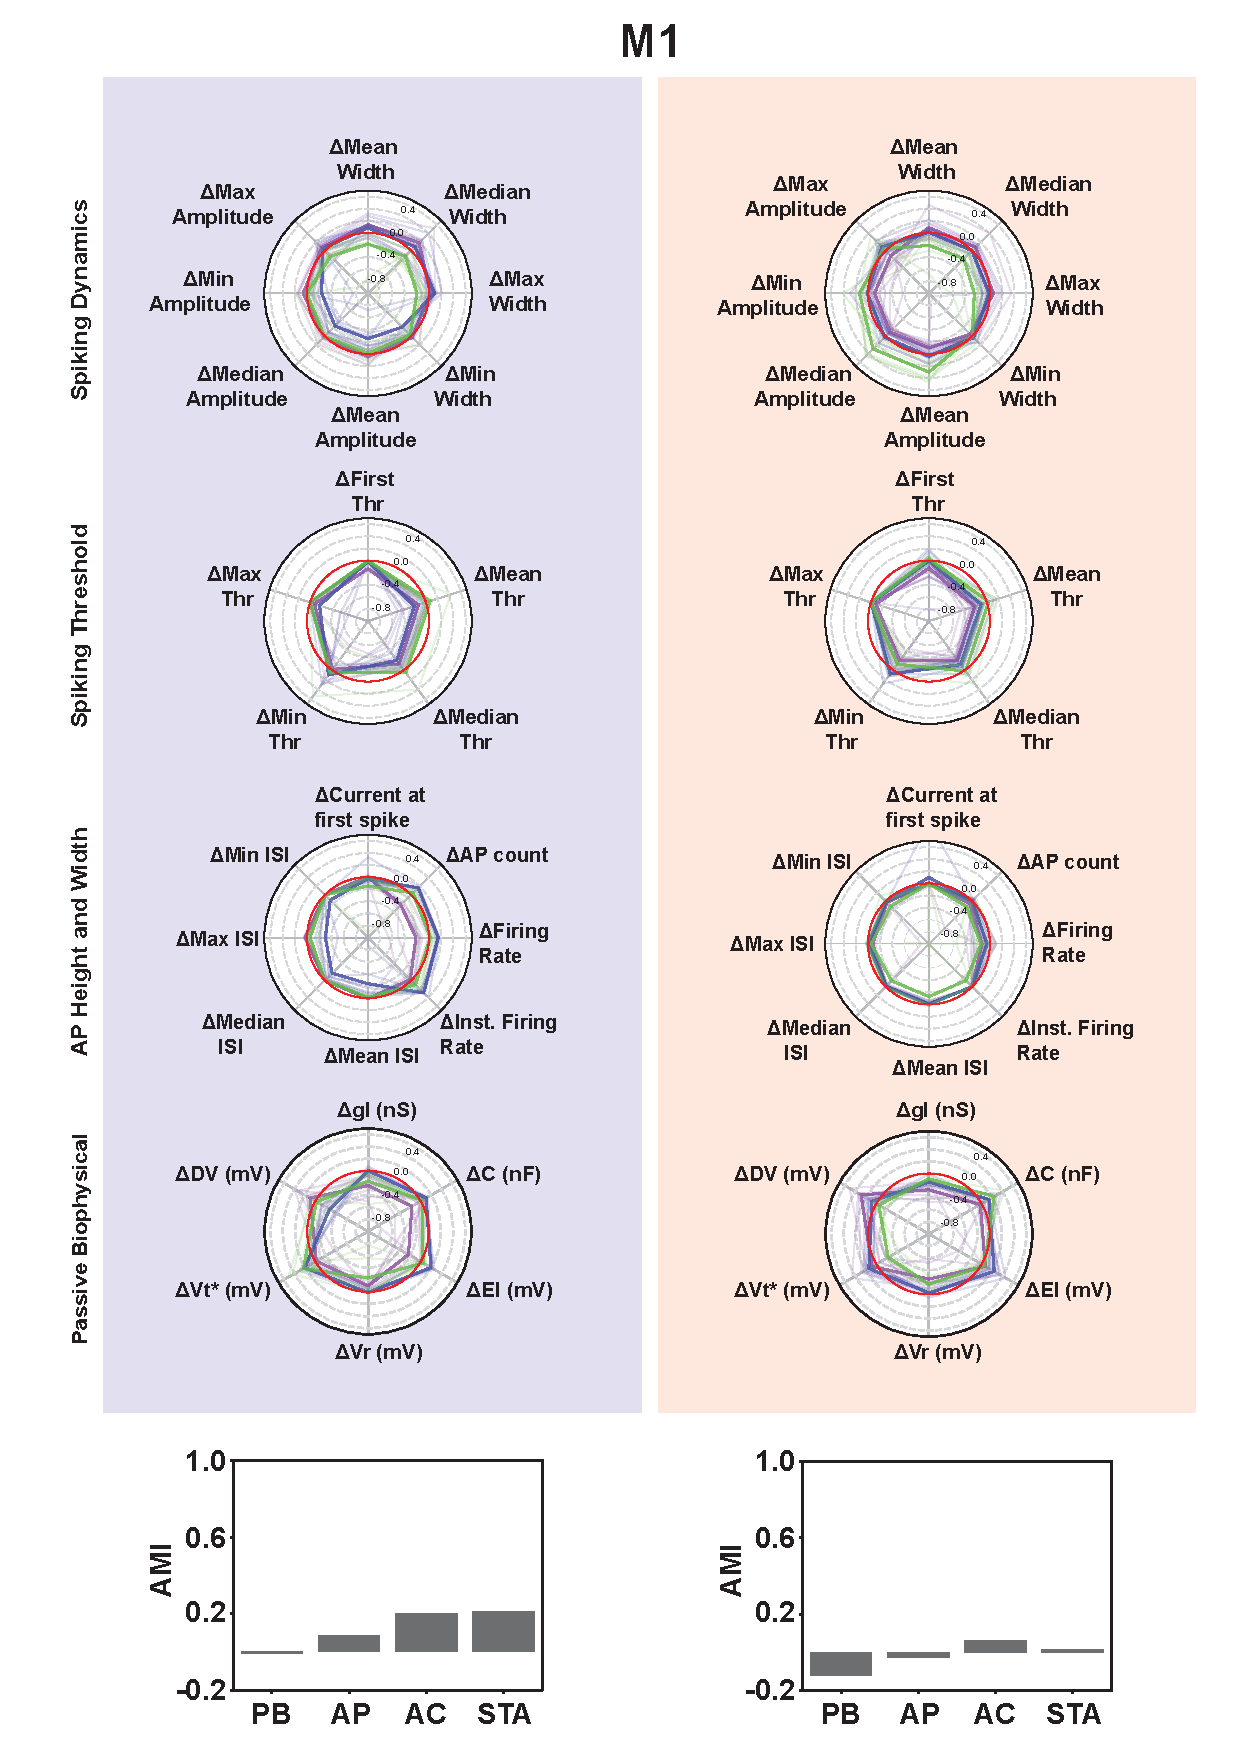
\includegraphics[width=0.9\linewidth]{Figures/Ch_3/Appendix9.pdf}
    \caption{\textbf{Clustering based on differences between control and M1 for action potential and passive biophysical attributes reveals subgroups of neurons getting modulated differently as a result of M1-R activation.}}
    \label{fig:S9}
\end{figure}


\newpage


\begin{figure}The polar plots show the clusters based on difference values between M1 and aCSF trials for action potential (subdivided into spiking dynamics, spiking threshold and AP height and width) and passive biophysical properties for both, excitatory (red background) and inhibitory (blue background). Each neuron is represented with a thin line and Coloured with their respective cluster label. The mean for each cluster is represented with a thick line. The histogram at the bottom shows the AMI score between cluster labels using aCSF trials and the cluster labels based on difference between M1 and aCSF trials.   
\end{figure}
\clearpage
\newpage
\begin{figure}
    \centering
    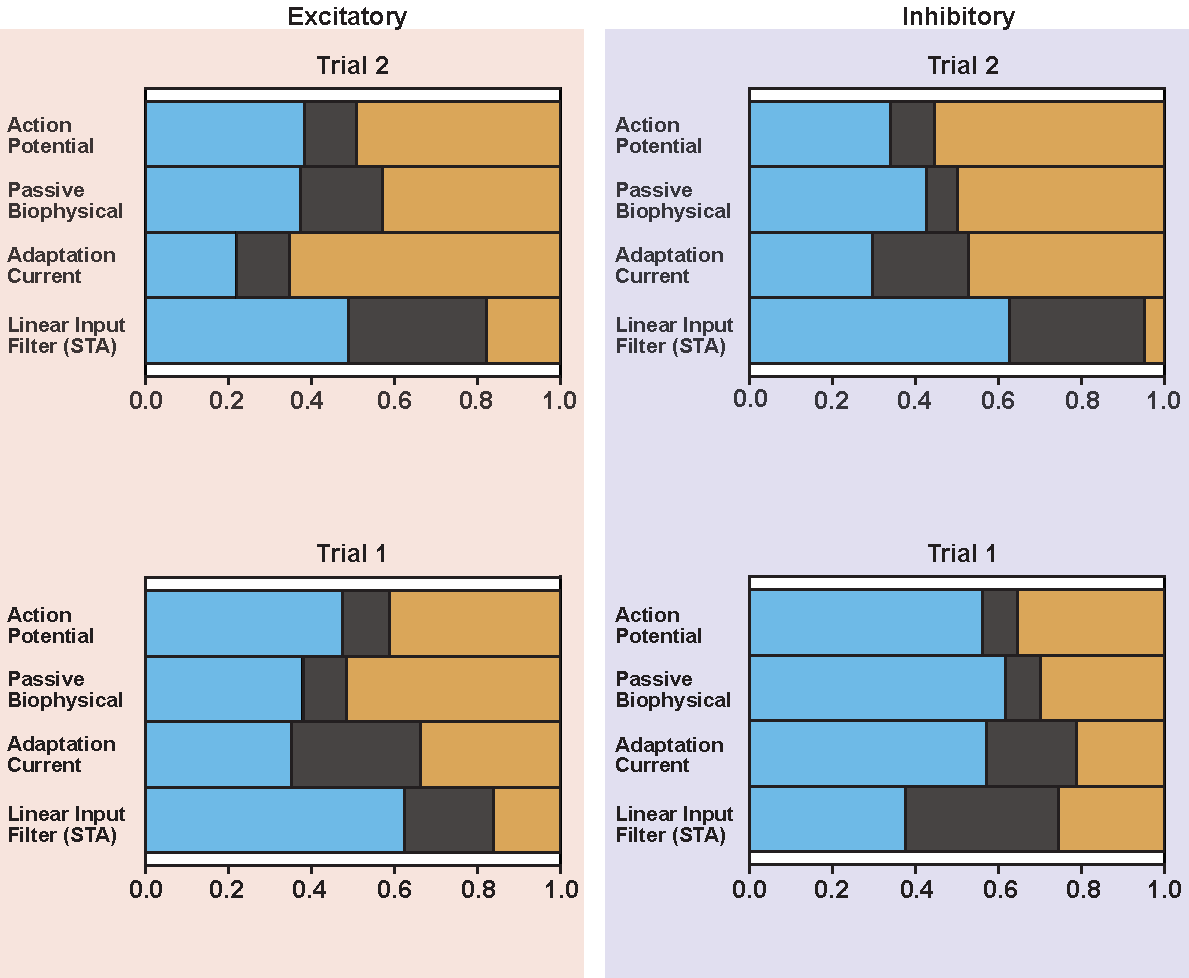
\includegraphics[width=0.9\linewidth]{Figures/Ch_3/Appendix10.pdf}
    \caption{\textbf{MCFA for 1st and 2nd aCSF trials.}}
    \label{fig:S10}
\end{figure}
\clearpage

\newpage

\begin{figure}
    \centering
    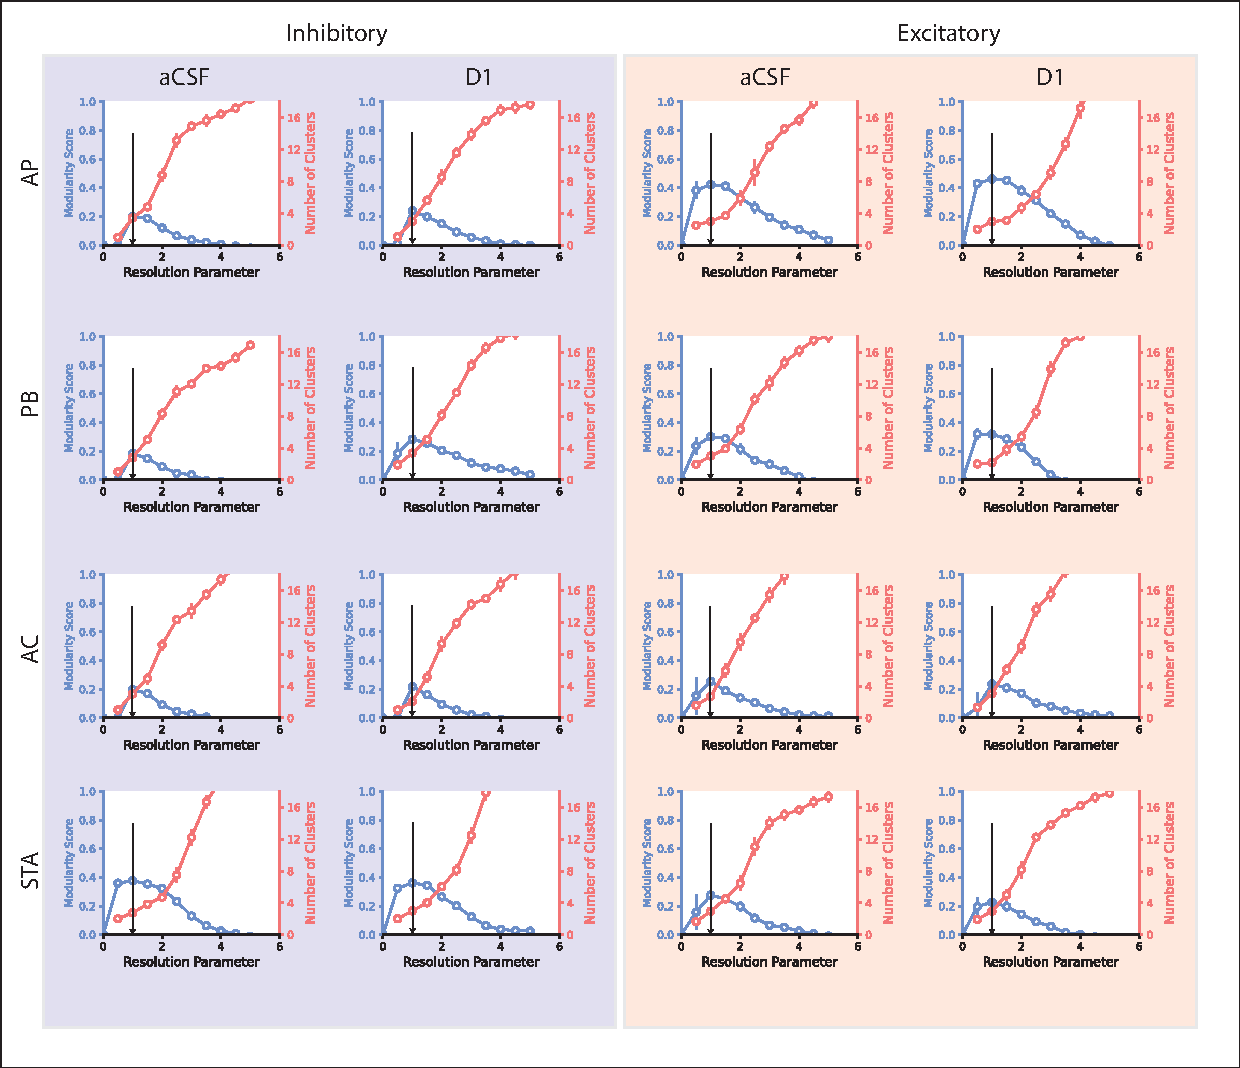
\includegraphics[width=\linewidth]{Figures/Ch_3/Appendix11.pdf}
    \caption{\textbf{Stability of clusters over a range of resolution parameters and the corresponding number of clusters for D1} The plot shows the modularity score for each resolution parameter and the corresponding number of clusters. The selected resolution parameter is marked with the black arrow, this corresponds to the highest modularity score.  }
    \label{fig:stability_d1}
\end{figure}
\clearpage

\begin{figure}
    \centering
    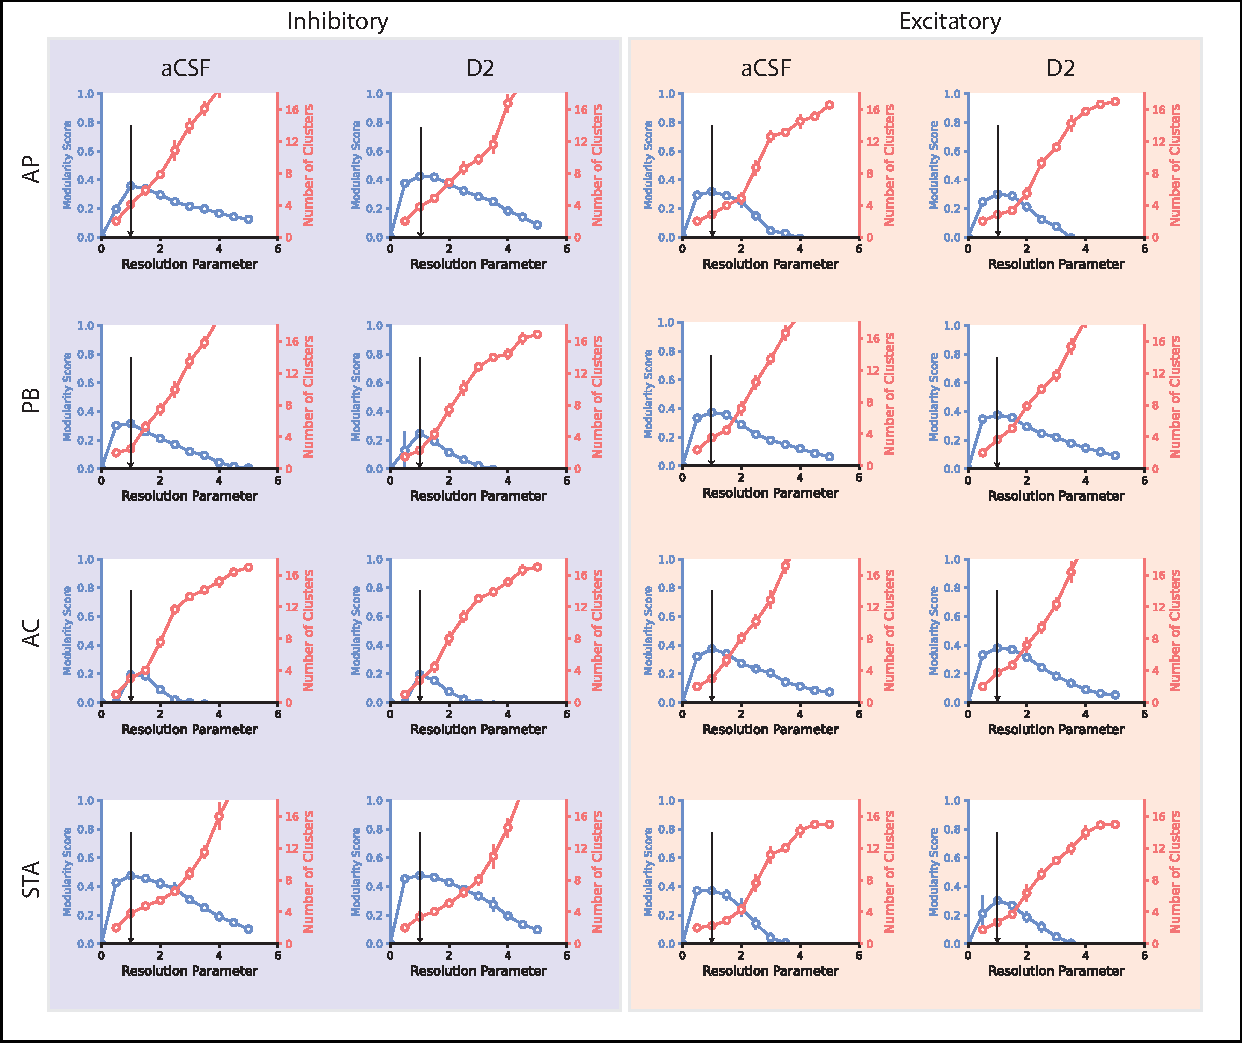
\includegraphics[width=\linewidth]{Figures/Ch_3/Appendix12.pdf}
    \caption{\textbf{Stability of clusters over a range of resolution parameters and the corresponding number of clusters for D2} The plot shows the modularity score for each resolution parameter and the corresponding number of clusters. The selected resolution parameter is marked with the black arrow, this corresponds to the highest modularity score.}
    \label{fig:stability_d2}
\end{figure}
\clearpage
\newpage

\begin{figure}
    \centering
    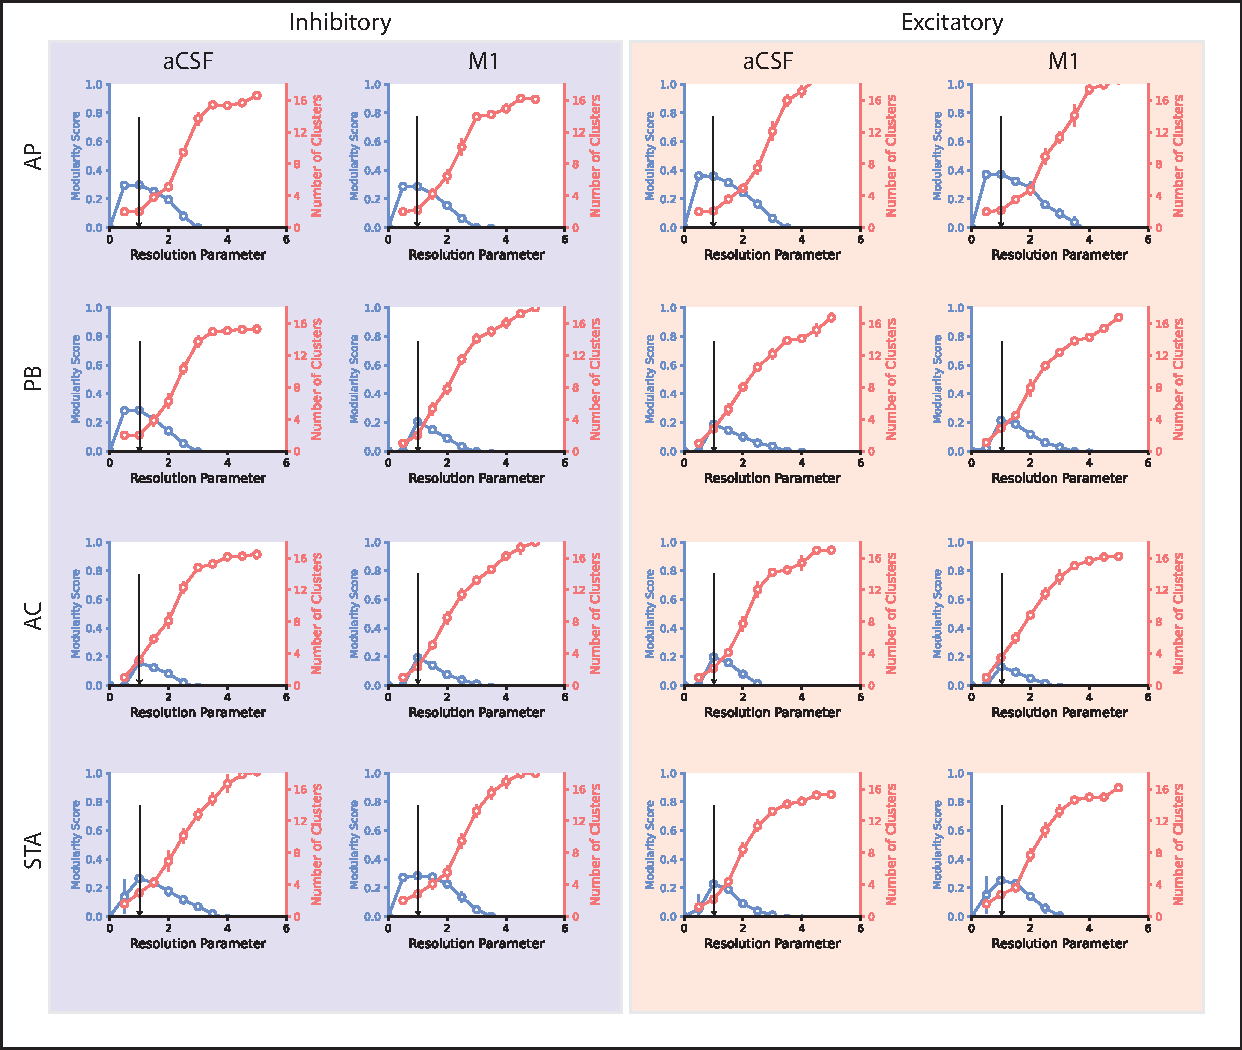
\includegraphics[width= \linewidth]{Figures/Ch_3/Appendix13.pdf}
    \caption{\textbf{Stability of clusters over a range of resolution parameters and the corresponding number of clusters for M1} The plot shows the modularity score for each resolution parameter and the corresponding number of clusters. The selected resolution parameter is marked with the black arrow, this corresponds to the highest modularity score.}
    \label{fig:stability_m1}
\end{figure}
\clearpage
\newpage
%%%%%%%%%%%%%%%% SUPPLEMENTARY TABLES %%%%%%%%%%%%%%%

\begin{table}[p]
\centering
\begin{tabular}{ccccc}
\hline
Condition         & Cell Type        & P‑value    & Statistic & Cohen’s \(d\)  \\
\hline 
D1–aCSF           & Inhibitory       & 0.019044   & 110       & –0.2409        \\
D1–aCSF           & Excitatory       & 0.104543   & 84        &  0.5385        \\
D2–aCSF           & Inhibitory       & 0.768005   & 87        & –0.0287        \\
D2–aCSF           & Excitatory       & 0.012016   & 225       &  0.3053        \\
M1–aCSF           & Inhibitory       & 0.523511   & 106       & –0.1181        \\
M1–aCSF           & Excitatory       & 0.002022   & 22        &  0.4790        \\
aCSF$_1$–aCSF$_2$ & Inhibitory       & 0.205410   & 170       & –0.3161        \\
aCSF$_1$–aCSF$_2$ & Excitatory       & 0.000111   & 340       &  0.3231        \\
\hline
\end{tabular}
\caption{Statistical comparison of fractional information (FI) changes under receptor activation.}
\label{tab:table1}
\end{table}
\clearpage
\newpage
%------------------------D1 ---------------------------------------------
% \newpage
    \begin{table}[p]
    \centering
    \begin{tabular}{llclllll}
        \hline
        Attribute & Variance type & aCSF &  D1 & D2 & M1 \\% 
        \hline
        AP  & Private   &  16.7742 (+/- 11.11)  & \textcolor{red}{0.0062}       & \textcolor{red}{0.1991}     &  \textcolor{red}{1.18E-03}     \\
        AP  & Shared    &  30.8543 (+/- 13.21)  & \textcolor{blue}{41.0578}     & \textcolor{blue}{55.0319}   &  \textcolor{blue}{66.0431}     \\
        AP  & Residual  &  52.3714 (+/- 12.18)  & \textcolor{blue}{58.9360}     & \textcolor{red}{44.7689}    &  \textcolor{red}{33.9556}      \\
        PB  & Private   &  18.5046 (+/- 13.50)  & \textcolor{red}{10.4084}      & \textcolor{red}{14.4461}    &  \textcolor{blue}{29.4316}      \\
        PB  & Shared    &  35.2320 (+/- 15.97)  & \textcolor{blue}{49.5931}     & \textcolor{red}{22.2190}    &  \textcolor{red}{26.3528}      \\
        PB  & Residual  &  46.2633 (+/- 15.84)  & \textcolor{red}{39.9985}      & \textcolor{blue}{63.2628}   &  \textcolor{red}{44.2155}      \\
        AC  & Private   &  18.0218 (+/- 17.14)  & \textcolor{red}{5.7216}       & \textcolor{red}{16.8436}    &  \textcolor{red}{10.3262}      \\
        AC  & Shared    &  15.8369 (+/- 11.35)  & \textcolor{red}{6.9056}       & \textcolor{blue}{30.6685}   &  \textcolor{blue}{35.0802}     \\
        AC  & Residual  &  66.1412 (+/- 21.22)  & \textcolor{blue}{87.3728}     & \textcolor{red}{44.7689}   &  \textcolor{red}{54.5935}     \\
        STA & Private   &  57.7380 (+/- 24.75)  & \textcolor{blue}{73.9663}     & \textcolor{blue}{71.2200}   &  \textcolor{red}{2.8344}       \\
        STA & Shared    &  23.6072 (+/- 19.86)  & \textcolor{red}{9.5260}       & \textcolor{red}{18.0047}   &  \textcolor{red}{6.9094}       \\
        STA & Residual  &  18.6546 (+/- 18.49)  & \textcolor{red}{16.5077}      & \textcolor{red}{10.7753}    &  \textcolor{blue}{90.2561}      \\     
        \hline
    \end{tabular}
    \caption{\textbf{Excitatory MCFA results}. Values that are reduced compared to bootstrapped aCSF are colored in red and values that are increased compared to aCSF are colored in blue. }
    \label{tab:specific_values_exc}
    \end{table}
\clearpage    
\newpage
\begin{table}[!htpb]
    \centering
    \begin{tabular}{llclllll}
        \hline
        Attribute & Variance type  & aCSF &  D1 & D2 & M1  \\
        \hline
        AP  & Private   & 14.9272 (+/- 09.5664)   &  \textcolor{red}{0.8297}     &  \textcolor{red}{1.6361}    &  \textcolor{red}{6.3213}       \\ 
        AP  & Shared    & 33.3099 (+/- 12.0733)   &  \textcolor{red}{32.3923}    &  \textcolor{red}{24.0248}   &  \textcolor{blue}{46.7960}    \\
        AP  & Residual  & 51.7627 (+/- 10.2972)   &  \textcolor{blue}{66.7777}   &  \textcolor{blue}{74.3390}  &  \textcolor{red}{46.8826}     \\
        PB  & Private   & 13.1228 (+/- 10.4672)   &  \textcolor{red}{3.9880}     &  \textcolor{red}{11.2795}   &  \textcolor{blue}{18.8554}    \\
        PB  & Shared    & 33.4015 (+/- 14.8031)   &  \textcolor{red}{25.2733}    &  \textcolor{blue}{53.6689}  &  \textcolor{blue}{51.5773}    \\
        PB  & Residual  & 53.4755 (+/- 15.0643)   &  \textcolor{blue}{70.7389}   &  \textcolor{red}{35.0514}   &  \textcolor{red}{29.5671}     \\
        AC  & Private   & 22.7058 (+/- 16.5534)   &  \textcolor{red}{11.6295}    &  \textcolor{blue}{26.3594}  &  \textcolor{blue}{50.6683}     \\
        AC  & Shared    & 26.9763 (+/- 14.6503)   &  \textcolor{blue}{44.4749}   &  \textcolor{blue}{38.9088}  &  \textcolor{red}{22.8306}    \\
        AC  & Residual  & 50.3177 (+/- 21.2265)   &  \textcolor{red}{43.8957}    &  \textcolor{red}{35.0514}   &  \textcolor{red}{26.5009}    \\
        STA & Private   & 55.1458 (+/- 25.8562)   &  \textcolor{red}{48.3895}    &  \textcolor{red}{21.5490}   &  \textcolor{red}{36.3625}    \\
        STA & Shared    & 23.6595 (+/- 17.2281)   &  \textcolor{blue}{46.2345}   &  \textcolor{blue}{66.6929}  &  \textcolor{blue}{54.3020}     \\   
        STA & Residual  & 21.1946 (+/- 21.2975)   &  \textcolor{red}{5.3761}     &  \textcolor{red}{11.7580}   &  \textcolor{red}{9.3353}       \\        
        \hline
    \end{tabular}
    \caption{\textbf{Inhibitory MCFA results}. Values that are reduced compared to bootstrapped aCSF are colored in red and values that are increased compared to aCSF are colored in blue. }
    \label{tab:specific_values_inh}
    \end{table}

\clearpage    
\newpage
    
    
\begin{table}[!htpb]
    \centering
    \begin{tabular}{llcc}
    \hline
    Attribute & Variance type  & Variance 1st Trial & Variance 2nd Trial \\
    \hline
    AP 	    & Private  &  11.2873 (+/- 11.81)	&\textcolor{blue}{12.4735 (+/- 08.39)}\\
    AP 	    & Shared   &  47.5009 (+/- 15.28)	&\textcolor{red}{38.4021 (+/- 10.44)}\\
    AP 	    & Residual &  41.2118 (+/- 10.25)	&\textcolor{blue}{49.1244 (+/- 08.84)}\\
    PB 	    & Private  &  10.3859 (+/- 08.94)	&\textcolor{blue}{19.9091 (+/- 12.32)}\\
    PB 	    & Shared   &  38.0565 (+/- 14.78)	&\textcolor{red}{37.3036 (+/- 14.24)}\\
    PB 	    & Residual &  51.5576 (+/- 18.05)	&\textcolor{red}{42.7873 (+/- 13.55)}\\
    AC 	    & Private  &  31.0247 (+/- 16.07)	&\textcolor{red}{12.7529 (+/- 09.86)}\\
    AC 	    & Shared   &  35.2139 (+/- 15.73)	&\textcolor{red}{22.0695 (+/- 11.62)}\\
    AC 	    & Residual &  33.7614 (+/- 14.71)	&\textcolor{blue}{65.1776 (+/- 16.40)}\\
    STA 	& Private  &  21.4966 (+/- 16.40)	&\textcolor{blue}{33.4581 (+/- 23.06)}\\
    STA 	& Shared   &  62.5138 (+/- 17.43)	&\textcolor{red}{48.8704 (+/- 25.72)}\\
    STA 	& Residual &  15.9897 (+/- 08.43)	&\textcolor{blue}{17.6716 (+/- 15.15)}\\
    \hline
    \end{tabular}
    \caption{\textbf{Excitatory MCFA results for second aCSF trial}. Values that are reduced compared to bootstrapped aCSF trial 1 are colored in red and values that are increased compared to aCSF trial 1 are colored in blue.}
    \label{tab:specific_values_exc_acsf}
    \end{table}
\clearpage    
\newpage    
\begin{table}[!htpb]
    \centering
    \begin{tabular}{llcc}
    \hline
    Attribute & Variance type  & Variance 1st Trial & Variance 2nd Trial \\
    \hline
    AP 	    & Private  &  08.4805 (+/- 07.68)  &	\textcolor{blue}{10.5232 (+/- 07.13)}\\
    AP 	    & Shared   &  56.1049 (+/- 11.24)  &	\textcolor{red}{33.9479 (+/- 17.05)} \\
    AP 	    & Residual &  35.4145 (+/- 07.97)  & 	\textcolor{blue}{55.5289 (+/- 18.73)}\\
    PB 	    & Private  &  08.3097 (+/- 06.94)  &	\textcolor{red}{07.4436 (+/- 09.55)}\\
    PB 	    & Shared   &  61.6040 (+/- 12.22)  &	\textcolor{red}{42.5329 (+/- 16.00)}\\
    PB 	    & Residual &  30.0864 (+/- 09.39)  & 	\textcolor{blue}{50.0235 (+/- 15.53)}\\
    AC 	    & Private  &  21.8111 (+/- 10.96)  &	\textcolor{blue}{23.1401 (+/- 15.18)}\\
    AC 	    & Shared   &  56.9907 (+/- 12.05)  &	\textcolor{red}{29.6210 (+/- 10.40)}\\
    AC 	    & Residual &  21.1982 (+/- 09.24)  & 	\textcolor{blue}{47.2389 (+/- 15.30)}\\
    STA 	& Private  &  36.8157 (+/- 23.86)  &	\textcolor{red}{32.6709 (+/- 21.86)}\\
    STA 	& Shared   &  37.5418 (+/- 17.49)  &	\textcolor{blue}{62.5230 (+/- 22.45)}\\
    STA 	& Residual &  25.6425 (+/- 22.69)   & 	\textcolor{red}{04.806 (+/- 02.85)}\\
    \hline
    \end{tabular}
    \caption{\textbf{Inhibitory MCFA results for second aCSF trial}. Values that are reduced compared to bootstrapped aCSF trial 1 are colored in red and values that are increased compared to aCSF trial 1 are colored in blue. }
    \label{tab:specific_values_inh_acsf}
    \end{table}


\newpage
\begin{spacing}{1.0} % Set the line spacing to single spacing
\fontsize{8pt}{8pt}\selectfont
\bibliographystyle{apalike} %%%%Changed
\renewcommand{\bibname}{References}
\bibliography{All_bibtex} %%%%Changed
\end{spacing}
% \printbibliography